% !TeX program = xelatex
% 编译：xelatex 08-卷积的性质.tex（VS Code 的 LaTeX Workshop 会读上一行，自动用 xelatex）
% 来源：2022 浙江大学《信号与系统》胡浩基老师，卷积的性质（两节课）。教材：分配律第 49 页；冲激偶第 14 页式 (1-48)、图 1-29；LTI 系统的稳定性第 52 页 2.3.2；因果性 2.3.3。
% 体例：先讲卷积的交换律、结合律、分配律，再记第二章的五个常用结论和一组冲激辨析题，最后讲 LTI 系统稳定、因果的充要条件。
\documentclass[UTF8,a4paper,11pt]{ctexart}
\usepackage{amsmath,amssymb}
\usepackage{geometry}
\geometry{margin=2.4cm}
\usepackage{xcolor}
\usepackage{mdframed}
\usepackage{booktabs}
\usepackage{needspace}
\usepackage{array}
\usepackage{enumitem}
\usepackage{tikz}
\usetikzlibrary{arrows.meta,positioning,calc,patterns}
\usepackage{float}
\usepackage{fancyhdr}
% 页眉页脚清空，只在右下角保留页号（含首页）
\fancypagestyle{plain}{%
  \fancyhf{}%
  \fancyfoot[R]{\thepage}%
  \renewcommand{\headrulewidth}{0pt}%
  \renewcommand{\footrulewidth}{0pt}}
\usepackage[hidelinks,unicode,bookmarksnumbered,bookmarksopen=true,bookmarksopenlevel=2,pdftitle={卷积的性质}]{hyperref}
\usepackage{bookmark}% XeTeX 下 hyperref 自带的大纲不生效，用 bookmark 宏包生成 PDF 书签（需编译两遍）

\setCJKmainfont{Songti SC}[BoldFont={Songti SC Bold}]
\setCJKsansfont{PingFang SC}

\newmdenv[backgroundcolor=blue!4,linecolor=blue!50!black,linewidth=1pt,innertopmargin=6pt,innerbottommargin=6pt]{rememberbox}
\newenvironment{remember}{\begin{rememberbox}\textbf{重点}\par\smallskip}{\end{rememberbox}}
\newmdenv[backgroundcolor=yellow!8,linecolor=orange!70!black,linewidth=1pt,innertopmargin=6pt,innerbottommargin=6pt]{notebox}
\newenvironment{note}{\begin{notebox}\textbf{说明}\par\smallskip}{\end{notebox}}

% ---------------------------------------------------------------- 画图用的小宏
% 坐标轴：\taxes[自变量名]{横轴起点}{横轴终点}{纵轴顶端}{纵轴底端}。原点标 0（放在左下，避开纵轴）。
\newcommand{\taxes}[5][t]{%
  \draw[->] (#2,0) -- (#3,0) node[right,font=\scriptsize] {$#1$};
  \draw[->] (0,#5) -- (0,#4);
  \node[anchor=north east,font=\tiny,gray!60!black,inner sep=1pt] at (0,-0.02) {$0$};}
% 横轴刻度 \xt{位置}{标签}（标在轴下方）、\xtu{位置}{标签}（标在轴上方，轴下方有曲线时用）、纵轴刻度 \yt{位置}{标签}：刻度线 + 白底数字。
\newcommand{\xt}[2]{\draw (#1,0) -- (#1,-0.1) node[anchor=north,font=\tiny,gray!60!black,fill=white,inner sep=0.6pt] {$#2$};}
\newcommand{\xtu}[2]{\draw (#1,0) -- (#1,0.1) node[anchor=south,font=\tiny,gray!60!black,fill=white,inner sep=0.6pt] {$#2$};}
\newcommand{\yt}[2]{\draw (0,#1) -- (-0.1,#1) node[anchor=east,font=\tiny,gray!60!black,fill=white,inner sep=0.6pt] {$#2$};}
% 冲激箭头 \imp{位置}{画出的高度}{强度标签}
\newcommand{\imp}[3]{\draw[->,ultra thick,red!70!black] (#1,0) -- (#1,#2);
  \node[anchor=south,font=\tiny,red!70!black,inner sep=1pt] at (#1,#2) {#3};}
% 两个图之间的运算符号
\newcommand{\opsym}[3]{\node[font=\Large] at (#1,#2) {#3};}
\tikzset{>=stealth,
  sig/.style={thick,blue!60!black},
  res/.style={thick,red!70!black},
  out/.style={thick,green!45!black},
  blk/.style={draw,thick,minimum width=1.2cm,minimum height=0.62cm,font=\small,fill=white},
  lab/.style={font=\small}}

% ---------------------------------------------------------------- 标题层级
\definecolor{secblue}{RGB}{31,78,121}
\definecolor{exorange}{RGB}{190,90,10}
\definecolor{ptteal}{RGB}{0,110,110}
\ctexset{
  section={format=\raggedright\Large\bfseries\color{secblue},
           beforeskip=3.2ex plus 1ex minus .5ex, afterskip=1.4ex,
           aftertitle={\par\nobreak\vspace{-1.1ex}\noindent\textcolor{secblue}{\rule{\linewidth}{0.8pt}}\par\nobreak\vspace{0.6ex}}},
  subsection={format=\raggedright\large\bfseries\color{secblue},
              beforeskip=2.4ex plus .8ex minus .4ex, afterskip=1.0ex}
}
% 例题标题：\example{标题}{结论}{附注}，附注一般留空。左边橙色实心「例 n」，右边结论标签；同时进 PDF 大纲（第 3 级）。
\newcounter{ex}[section]
\newcommand{\example}[3]{%
  \refstepcounter{ex}\phantomsection
  \addcontentsline{toc}{subsubsection}{例 \theex\ #1（#2）}%
  \par\addvspace{1.6ex}\noindent
  {\setlength{\fboxsep}{3pt}%
   \colorbox{exorange}{\textcolor{white}{\textbf{例~\theex}}}\ %
   \textcolor{exorange}{\textbf{#1}}\ {\footnotesize\textcolor{gray!70!black}{#3}}%
   \hfill\colorbox{exorange!12}{\small\textcolor{exorange}{#2}}\par}%
  \nobreak\vskip0.6ex\relax\csname @afterheading\endcsname}
% 小标题（接着同一段往下写，不进大纲）：青色三角 + 粗体。
\newcommand{\point}[1]{\par\addvspace{1ex}\noindent\textcolor{ptteal}{$\blacktriangleright$\,\textbf{#1}}\ }

\title{卷积的性质\\\large 浙江大学 2022《信号与系统》（胡浩基）第二章听课笔记（教材第 49、52 页）}
\author{}
\date{}

\begin{document}
\pagestyle{plain}
\maketitle

%==================================================================
\section{交换律}\label{sec:comm}
\begin{remember}
卷积满足交换律(commutative property)：
\[
x(t)\ast h(t)=h(t)\ast x(t),\qquad x[n]\ast h[n]=h[n]\ast x[n].
\]
离散的情况只是把所有的圆括号 $(t)$ 换成方括号 $[n]$、积分换成求和，下面的性质都是如此。
\end{remember}

\point{证明（连续）。}
\begin{align*}
x(t)\ast h(t)&=\int_{-\infty}^{+\infty}x(\tau)\,h(t-\tau)\,\mathrm{d}\tau .
\end{align*}
设 $\tau'=t-\tau$，则 $\tau=t-\tau'$，$\mathrm{d}\tau=-\mathrm{d}\tau'$；$\tau$ 从 $-\infty$ 到 $+\infty$ 时，$\tau'$ 从 $+\infty$ 到 $-\infty$。负号用来把上下限换回来：
\begin{align*}
x(t)\ast h(t)&=\int_{+\infty}^{-\infty}x(t-\tau')\,h(\tau')\,(-\mathrm{d}\tau')\\
&=\int_{-\infty}^{+\infty}h(\tau')\,x(t-\tau')\,\mathrm{d}\tau'\\
&=h(t)\ast x(t).
\end{align*}
离散的情况设 $k'=n-k$，推法相同。第 06 篇证明「勒贝格意义下相等的两个函数，与任何函数卷积的结果都相同」时已经用到了交换律。

\point{用系统来说。}$h(t)$ 是 LTI 系统的冲激响应(impulse response)，也叫系统函数。交换律说的是：输入信号和冲激响应的角色可以对调，输出不变。

\begin{figure}[H]
\centering
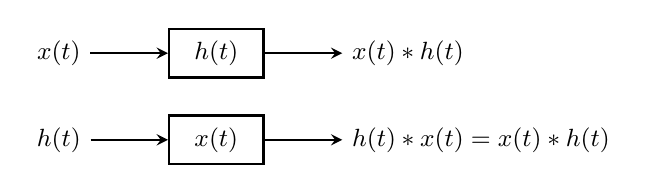
\begin{tikzpicture}
  \node[lab] (a1) at (0,0) {$x(t)$};
  \node[blk] (b1) at (2,0) {$h(t)$};
  \node[lab,anchor=west] (c1) at (3.6,0) {$x(t)\ast h(t)$};
  \draw[->,thick] (a1) -- (b1); \draw[->,thick] (b1) -- (c1);
  \node[lab] (a2) at (0,-1.1) {$h(t)$};
  \node[blk] (b2) at (2,-1.1) {$x(t)$};
  \node[lab,anchor=west] (c2) at (3.6,-1.1) {$h(t)\ast x(t)=x(t)\ast h(t)$};
  \draw[->,thick] (a2) -- (b2); \draw[->,thick] (b2) -- (c2);
\end{tikzpicture}
\caption{上：$x(t)$ 输入冲激响应为 $h(t)$ 的系统。下：$h(t)$ 输入冲激响应为 $x(t)$ 的系统。两者输出相同。}
\end{figure}

\point{图解法的理解：镜子两边。}图解法算 $x\ast h$，是把 $h$ 翻转、平移，与不动的 $x$ 相乘再积分。设想 $x$、$h$ 画在一块透明的板上：从正面看是 $h$ 被翻转；绕到背面看，同一幅图变成 $x$ 被翻转、$h$ 没翻转。再者运动是相对的：$h$ 向右滑过 $x$，等价于 $h$ 不动、$x$ 向左滑过 $h$。两种看法下每一时刻重叠部分的面积都一样，所以交换律天然成立。这种理解不区分连续和离散。

\begin{figure}[H]
\centering
\begin{tikzpicture}[x=1.15cm,y=1.3cm]
  \begin{scope}
    \fill[orange!25] (0.5,0) -- (1.5,1) -- (1.5,0) -- cycle;
    \taxes[\tau]{-1}{3.2}{1.45}{-0.2}
    \draw[sig] (-0.9,0) -- (0,0) -- (0,1) -- (2,1) -- (2,0) -- (3,0);
    \draw[res] (0.5,0) -- (1.5,1) -- (1.5,0);
    \xt{0.5}{0.5}\xt{1.5}{1.5}\xt{2}{2}\yt{1}{1}
    \node[font=\footnotesize,blue!60!black,anchor=south] at (1.0,1.0) {$x(\tau)$};
    \node[font=\footnotesize,red!70!black,anchor=west] at (2.0,0.55) {$h(1.5-\tau)$};
    \node[font=\footnotesize,anchor=west] at (-1,1.75) {$x\ast h$：$h$ 翻转};
  \end{scope}
  \begin{scope}[shift={(6.0,0)}]
    \fill[orange!25] (0,0) -- (0,1) -- (1,0) -- cycle;
    \taxes[\tau]{-1}{3.2}{1.45}{-0.2}
    \draw[res,dashed] (-0.9,0) -- (-0.5,0) -- (-0.5,1) -- (1.5,1) -- (1.5,0) -- (3,0);
    \draw[sig] (0,0) -- (0,1) -- (1,0);
    \xt{-0.5}{-0.5}\xt{1}{1}\xt{1.5}{1.5}\yt{1}{1}
    \node[font=\footnotesize,blue!60!black,anchor=west] at (0.55,0.55) {$h(\tau)$};
    \node[font=\footnotesize,red!70!black,anchor=south] at (1.5,1.0) {$x(1.5-\tau)$};
    \node[font=\footnotesize,anchor=west] at (-1,1.75) {$h\ast x$：$x$ 翻转};
  \end{scope}
\end{tikzpicture}
\caption{取 $x(t)$ 为 $[0,2]$ 上高 $1$ 的方波，$h(t)=1-t\ (0\le t\le1)$，看 $t=1.5$ 时刻。左：翻转 $h$，重叠面积为 $\frac12$；右：翻转 $x$，重叠面积也是 $\frac12$。}
\end{figure}

\point{取值范围也一致。}$y(t)$ 的最左端 $=$ $x$ 的最左端 $+$ $h$ 的最左端 $=$ $h$ 的最左端 $+$ $x$ 的最左端，最右端同理。交换以后 $y(t)$ 的取值范围不变。

%==================================================================
\section{结合律}\label{sec:assoc}
\begin{remember}
结合律(associative property)：
\[
\big[x(t)\ast h_1(t)\big]\ast h_2(t)=\big[x(t)\ast h_2(t)\big]\ast h_1(t).
\]
这里写成「交换两个系统的先后次序」的形式，与教材的写法 $[x\ast h_1]\ast h_2=x\ast[h_1\ast h_2]$ 核心意思一致。\textbf{交换律加结合律：多个信号做卷积，可以任意调换次序，结果不变}，例如
\[
x_1(t)\ast x_2(t)\ast x_3(t)\ast x_4(t)=x_2(t)\ast x_3(t)\ast x_1(t)\ast x_4(t).
\]
\end{remember}

\subsection{证法一：二重积分换元}
\point{写出左边。}先算里层，记
\[
z(t)=x(t)\ast h_1(t)=\int_{-\infty}^{+\infty}x(\tau_1)\,h_1(t-\tau_1)\,\mathrm{d}\tau_1 .
\]
外层积分变量已经叫 $\tau$，里层不能再叫 $\tau$，否则代入后两个 $\tau$ 混在一起，所以引入新的积分变量 $\tau_1$。于是
\begin{align*}
\big[x(t)\ast h_1(t)\big]\ast h_2(t)&=z(t)\ast h_2(t)=\int_{-\infty}^{+\infty}z(\tau)\,h_2(t-\tau)\,\mathrm{d}\tau\\
&=\int_{-\infty}^{+\infty}\left[\int_{-\infty}^{+\infty}x(\tau_1)\,h_1(\tau-\tau_1)\,\mathrm{d}\tau_1\right]h_2(t-\tau)\,\mathrm{d}\tau .
\end{align*}
\point{右边。}把 $h_1$、$h_2$ 对调即可，要证明左边等于
\[
\int_{-\infty}^{+\infty}\left[\int_{-\infty}^{+\infty}x(\tau_1)\,h_2(\tau-\tau_1)\,\mathrm{d}\tau_1\right]h_1(t-\tau)\,\mathrm{d}\tau .
\]
\point{同时换两个元。}左边是对 $\tau_1$、$\tau$ 的二重积分，设
\[
\tau_1'=\tau_1,\qquad \tau'=t+\tau_1-\tau .
\]
雅可比行列式(Jacobian determinant)为
\[
\frac{\partial(\tau',\tau_1')}{\partial(\tau,\tau_1)}=
\begin{vmatrix}\dfrac{\partial\tau'}{\partial\tau}&\dfrac{\partial\tau'}{\partial\tau_1}\\[2ex]\dfrac{\partial\tau_1'}{\partial\tau}&\dfrac{\partial\tau_1'}{\partial\tau_1}\end{vmatrix}
=\begin{vmatrix}-1&1\\0&1\end{vmatrix}=-1,
\]
绝对值为 $1$，所以 $\mathrm{d}\tau_1\,\mathrm{d}\tau=\mathrm{d}\tau_1'\,\mathrm{d}\tau'$，积分区域仍是整个平面。代入
\[
\tau-\tau_1=t-\tau',\qquad t-\tau=\tau'-\tau_1',
\]
左边变成
\[
\int_{-\infty}^{+\infty}\!\!\int_{-\infty}^{+\infty}x(\tau_1')\,h_1(t-\tau')\,h_2(\tau'-\tau_1')\,\mathrm{d}\tau_1'\,\mathrm{d}\tau' .
\]
去掉所有的撇号，逐项对照：$x(\tau_1)$ 对 $x(\tau_1)$，$h_1(t-\tau)$ 对 $h_1(t-\tau)$，$h_2(\tau-\tau_1)$ 对 $h_2(\tau-\tau_1)$，正好是右边。证毕。

\subsection{证法二：用系统来证}
这个证法不区分连续和离散。把等式两边看成两个系统的输出：

\begin{figure}[H]
\centering
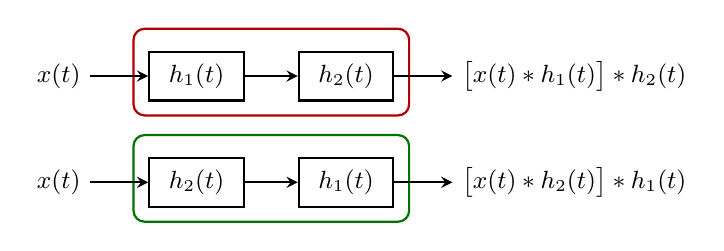
\begin{tikzpicture}
  \draw[red!70!black,thick,rounded corners] (0.95,-0.5) rectangle (4.45,0.6);
  \node[lab] (a1) at (0,0) {$x(t)$};
  \node[blk] (b1) at (1.75,0) {$h_1(t)$};
  \node[blk] (c1) at (3.65,0) {$h_2(t)$};
  \node[lab,anchor=west] (d1) at (5.0,0) {$\big[x(t)\ast h_1(t)\big]\ast h_2(t)$};
  \draw[->,thick] (a1) -- (b1); \draw[->,thick] (b1) -- (c1); \draw[->,thick] (c1) -- (d1);
  \draw[green!45!black,thick,rounded corners] (0.95,-1.85) rectangle (4.45,-0.75);
  \node[lab] (a2) at (0,-1.35) {$x(t)$};
  \node[blk] (b2) at (1.75,-1.35) {$h_2(t)$};
  \node[blk] (c2) at (3.65,-1.35) {$h_1(t)$};
  \node[lab,anchor=west] (d2) at (5.0,-1.35) {$\big[x(t)\ast h_2(t)\big]\ast h_1(t)$};
  \draw[->,thick] (a2) -- (b2); \draw[->,thick] (b2) -- (c2); \draw[->,thick] (c2) -- (d2);
\end{tikzpicture}
\caption{红框：先过 $h_1$ 再过 $h_2$；绿框：先过 $h_2$ 再过 $h_1$。只要证明红框和绿框是同一个系统，结合律就成立。}
\end{figure}

\point{引理：两个 LTI 系统串联(cascade)或并联(parallel)，仍是 LTI 系统。}用齐次性(homogeneity)、叠加性(additivity)和时不变性逐条验证。

\begin{figure}[H]
\centering
\begin{tikzpicture}
  \node[lab] (x) at (0,0) {$x(t)$};
  \node[blk] (p) at (1.8,0) {LTI\,1};
  \node[blk] (q) at (4.0,0) {LTI\,2};
  \node[lab,anchor=west] (y) at (5.3,0) {$y(t)$};
  \draw[->,thick] (x) -- (p); \draw[->,thick] (p) -- node[above,font=\scriptsize]{$z(t)$} (q); \draw[->,thick] (q) -- (y);
  \node[font=\footnotesize] at (2.9,-0.75) {串联};
  \begin{scope}[shift={(7.6,0)}]
    \node[lab] (x2) at (0,0) {$x(t)$};
    \coordinate (s) at (0.8,0);
    \node[blk] (p2) at (2.1,0.6) {LTI\,1};
    \node[blk] (q2) at (2.1,-0.6) {LTI\,2};
    \node[draw,thick,circle,inner sep=1pt] (sum) at (3.9,0) {$+$};
    \node[lab,anchor=west] (y2) at (4.5,0) {$y(t)$};
    \draw[thick] (x2) -- (s); \fill (s) circle (1.3pt);
    \draw[->,thick] (s) |- (p2); \draw[->,thick] (s) |- (q2);
    \draw[->,thick] (p2) -| node[pos=0.3,above,font=\scriptsize]{$z_1(t)$} (sum);
    \draw[->,thick] (q2) -| node[pos=0.3,below,font=\scriptsize]{$z_2(t)$} (sum);
    \draw[->,thick] (sum) -- (y2);
    \node[font=\footnotesize] at (2.1,-1.25) {并联：$y=z_1+z_2$};
  \end{scope}
\end{tikzpicture}
\caption{两个 LTI 系统的串联与并联，合起来仍是一个 LTI 系统。}
\end{figure}

串联：设 $x\to z\to y$。
\begin{itemize}[nosep]
\item 齐次性：输入 $a\,x$，由 LTI\,1 得中间信号 $a\,z$，再由 LTI\,2 得 $a\,y$。
\item 叠加性：输入 $x_1+x_2$，由 LTI\,1 得 $z_1+z_2$，再由 LTI\,2 得 $y_1+y_2$。
\item 时不变：输入 $x(t-t_0)$，中间信号为 $z(t-t_0)$，输出为 $y(t-t_0)$。
\end{itemize}
并联：$y=z_1+z_2$。
\begin{itemize}[nosep]
\item 齐次性：输入 $a\,x$，两路分别得 $a\,z_1$、$a\,z_2$，相加得 $a\,y$。
\item 叠加性：记 $z_{ij}$ 为第 $i$ 路对 $x_j$ 的输出。输入 $x_1+x_2$，第 1 路得 $z_{11}+z_{12}$，第 2 路得 $z_{21}+z_{22}$，相加并重新分组：$(z_{11}+z_{21})+(z_{12}+z_{22})=y_1+y_2$。
\item 时不变：两路都平移 $t_0$，相加后仍平移 $t_0$。
\end{itemize}

\point{两个 LTI 系统相同，只需冲激响应相同。}冲激响应唯一确定 LTI 系统（第 05 篇）：输入 $\delta(t)$ 的输出一样，则对所有输入的输出都一样。由引理，红框、绿框都是 LTI 系统。输入 $\delta(t)$：
\begin{align*}
\text{红框：}&\ \big[\delta(t)\ast h_1(t)\big]\ast h_2(t)=h_1(t)\ast h_2(t),\\
\text{绿框：}&\ \big[\delta(t)\ast h_2(t)\big]\ast h_1(t)=h_2(t)\ast h_1(t).
\end{align*}
由交换律，两者相等。所以红框和绿框是同一个系统，对任意 $x(t)$ 输出都相同，结合律得证。

%==================================================================
\section{分配律}\label{sec:dist}
\begin{remember}
卷积满足分配律(distributive property)（教材第 49 页）：
\begin{align*}
x(t)\ast\big[h_1(t)+h_2(t)\big]&=x(t)\ast h_1(t)+x(t)\ast h_2(t),\\
x[n]\ast\big(h_1[n]+h_2[n]\big)&=x[n]\ast h_1[n]+x[n]\ast h_2[n].
\end{align*}
\end{remember}
原因一句话：积分与求和本身满足分配律，
\[
\int_{-\infty}^{+\infty}x(\tau)\big[h_1(t-\tau)+h_2(t-\tau)\big]\mathrm{d}\tau
=\int_{-\infty}^{+\infty}x(\tau)h_1(t-\tau)\,\mathrm{d}\tau+\int_{-\infty}^{+\infty}x(\tau)h_2(t-\tau)\,\mathrm{d}\tau .
\]
用系统来说：两个系统并联，等于一个冲激响应为 $h_1+h_2$ 的系统。

\begin{figure}[H]
\centering
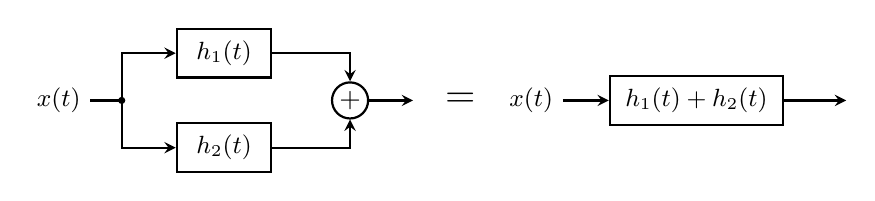
\begin{tikzpicture}
  \node[lab] (x2) at (0,0) {$x(t)$};
  \coordinate (s) at (0.8,0);
  \node[blk] (p2) at (2.1,0.6) {$h_1(t)$};
  \node[blk] (q2) at (2.1,-0.6) {$h_2(t)$};
  \node[draw,thick,circle,inner sep=1pt] (sum) at (3.7,0) {$+$};
  \draw[thick] (x2) -- (s); \fill (s) circle (1.3pt);
  \draw[->,thick] (s) |- (p2); \draw[->,thick] (s) |- (q2);
  \draw[->,thick] (p2) -| (sum); \draw[->,thick] (q2) -| (sum);
  \draw[->,thick] (sum) -- (4.5,0);
  \node[font=\Large] at (5.1,0) {$=$};
  \node[lab] (x3) at (6.0,0) {$x(t)$};
  \node[blk,minimum width=2.2cm] (b3) at (8.1,0) {$h_1(t)+h_2(t)$};
  \draw[->,thick] (x3) -- (b3); \draw[->,thick] (b3) -- (10.0,0);
\end{tikzpicture}
\caption{并联的两个系统，相当于冲激响应相加后的一个系统。}
\end{figure}

\begin{note}
交换律、结合律、分配律合起来：多个信号的卷积可以任意调换次序；与加法混在一起时可以像乘法那样展开。
\end{note}

%==================================================================
\needspace{14\baselineskip}
\section{第二章的五个常用结论}\label{sec:tips}

\subsection{方波写成阶跃之差}\label{sub:rect}
\begin{remember}
从 $a$ 到 $b$、高为 $1$ 的方波：
\[
u(t-a)-u(t-b).
\]
\end{remember}

\example{两个方波的卷积}{\texorpdfstring{$[0,4]$ 上高为 2 的三角波}{[0,4] 上的三角波}}{}
\textbf{题目}：求 $\big[u(t-1)-u(t-3)\big]\ast\big[u(t+1)-u(t-1)\big]$。

\point{先认出方波。}第一项是 $[1,3]$ 上的方波，第二项是 $[-1,1]$ 上的方波，两个宽度都是 $2$、高度都是 $1$，卷积结果是三角波（第 07 篇等宽方波的结论）。

\point{取值范围与峰值。}起点 $1+(-1)=0$，终点 $3+1=4$；峰值在中点 $t=2$，等于两方波完全重叠时的面积 $2\times1\times1=2$。

\begin{figure}[H]
\centering
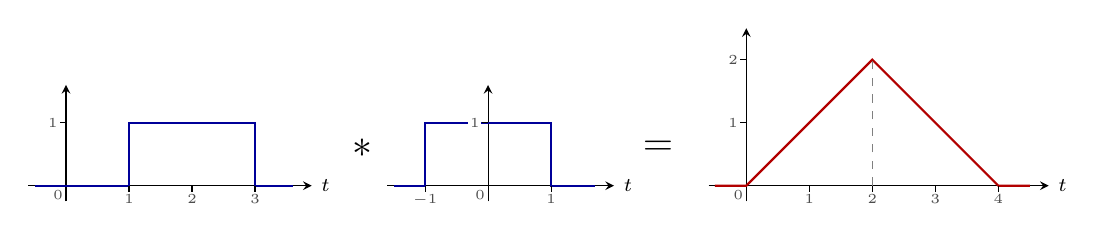
\begin{tikzpicture}[x=0.8cm,y=0.8cm]
  \begin{scope}
    \taxes{-0.6}{3.9}{1.6}{-0.25}
    \draw[sig] (-0.5,0) -- (1,0) -- (1,1) -- (3,1) -- (3,0) -- (3.6,0);
    \xt{1}{1}\xt{2}{2}\xt{3}{3}\yt{1}{1}
  \end{scope}
  \opsym{4.7}{0.6}{$\ast$}
  \begin{scope}[shift={(6.7,0)}]
    \taxes{-1.6}{2.0}{1.6}{-0.25}
    \draw[sig] (-1.5,0) -- (-1,0) -- (-1,1) -- (1,1) -- (1,0) -- (1.7,0);
    \xt{-1}{-1}\xt{1}{1}\yt{1}{1}
  \end{scope}
  \opsym{9.4}{0.6}{$=$}
  \begin{scope}[shift={(10.8,0)}]
    \taxes{-0.6}{4.8}{2.5}{-0.25}
    \draw[res] (-0.5,0) -- (0,0) -- (2,2) -- (4,0) -- (4.5,0);
    \draw[dashed,gray] (2,0) -- (2,2);
    \xt{1}{1}\xt{2}{2}\xt{3}{3}\xt{4}{4}\yt{1}{1}\yt{2}{2}
  \end{scope}
\end{tikzpicture}
\caption{$[1,3]$ 上的方波卷 $[-1,1]$ 上的方波，得到 $[0,4]$ 上、峰值为 $2$（在 $t=2$）的三角波。}
\end{figure}

\point{易错点。}这类题的关键是先把阶跃之差认成方波，再用图解法。若直接用分配律拆成四项阶跃卷积，计算繁琐、容易出错（拆开后的做法见 \ref{sub:shift} 小节末尾的验算）。

\subsection{与阶跃卷积：积分器与累加器}\label{sub:step}
\begin{remember}
与阶跃卷积，就是从 $-\infty$ 积分（累加）到当前时刻：
\[
x(t)\ast u(t)=\int_{-\infty}^{t}x(\tau)\,\mathrm{d}\tau,\qquad
x[n]\ast u[n]=\sum_{k=-\infty}^{n}x[k].
\]
冲激响应为 $u(t)$ 的系统是积分器(integrator)，冲激响应为 $u[n]$ 的系统是累加器(accumulator)。后面的章节常用。
\end{remember}

\point{证明。}
\[
x(t)\ast u(t)=\int_{-\infty}^{+\infty}x(\tau)\,u(t-\tau)\,\mathrm{d}\tau .
\]
$u(t-\tau)$ 只在 $t-\tau>0$，即 $\tau<t$ 时等于 $1$，其余为 $0$。积分上下限是对 $\tau$ 而言的，所以只剩 $\tau$ 从 $-\infty$ 到 $t$ 的部分：
\[
x(t)\ast u(t)=\int_{-\infty}^{t}x(\tau)\,\mathrm{d}\tau .
\]
离散的情况同理，$u[n-k]$ 只在 $k\le n$ 时为 $1$。

\point{图解法的理解。}把 $u(\tau)$ 翻转成 $u(-\tau)$，它覆盖整个左半轴；再平移到 $t$，就把 $x$ 在 $t$ 左边的部分全部框住，积分就是从 $-\infty$ 积到 $t$。

\begin{figure}[H]
\centering
\begin{tikzpicture}[x=1.1cm,y=1.6cm]
  \fill[blue!12] (-3.2,0) -- plot[domain=-3.2:1.5,samples=60] (\x,{0.6+0.3*sin(1.2*\x r)}) -- (1.5,0) -- cycle;
  \taxes[\tau]{-3.4}{4.4}{1.5}{-0.2}
  \draw[sig,domain=-3.3:4.2,samples=80] plot (\x,{0.6+0.3*sin(1.2*\x r)});
  \draw[res,dashed] (-3.3,1.2) -- (1.5,1.2) -- (1.5,0);
  \draw[res,dashed] (1.5,0) -- (4.2,0);
  \xt{1.5}{t}\yt{1.2}{1}
  \node[font=\footnotesize,red!70!black,anchor=south west] at (-3.3,1.22) {$u(t-\tau)$：$\tau<t$ 时为 $1$};
  \node[font=\footnotesize,blue!60!black,anchor=west] at (2.4,0.85) {$x(\tau)$};
  \node[font=\footnotesize,anchor=east] at (-3.4,0.6) {$\cdots$};
\end{tikzpicture}
\caption{$u(t-\tau)$ 把 $x(\tau)$ 在 $\tau<t$ 的部分全部框住，阴影面积就是 $x(t)\ast u(t)=\int_{-\infty}^{t}x(\tau)\,\mathrm{d}\tau$。}
\end{figure}

\subsection{冲激偶函数}\label{sub:doublet}
\begin{remember}
冲激偶(unit doublet)是冲激函数的导数（教材第 14 页，图 1-29）：
\[
\delta'(t)=\frac{\mathrm{d}\,\delta(t)}{\mathrm{d}t}.
\]
它的性质（教材式 (1-48)）：
\[
\int_{-\infty}^{+\infty}x(t)\,\delta'(t)\,\mathrm{d}t=-x'(0).
\]
\end{remember}

\point{形状。}$\delta(t)$ 是宽 $\Delta$、高 $\frac1\Delta$ 的方波 $\delta_\Delta(t)$ 在 $\Delta\to0$ 时的极限。$\delta_\Delta(t)$ 在 $t=0$ 处向上跳 $\frac1\Delta$，求导得强度为 $\frac1\Delta$ 的正冲激；在 $t=\Delta$ 处向下跳 $\frac1\Delta$，求导得强度为 $\frac1\Delta$ 的负冲激。$\Delta\to0$ 时，两者合到原点：左侧（左极限处）向上无限大，右侧（右极限处）向下无限大。

\begin{figure}[H]
\centering
\begin{tikzpicture}[x=1.15cm,y=0.75cm]
  \begin{scope}
    \taxes{-1}{2.1}{2.6}{-0.3}
    \draw[sig] (-0.9,0) -- (0,0) -- (0,1.8) -- (0.6,1.8) -- (0.6,0) -- (1.9,0);
    \xt{0.6}{\Delta}\yt{1.8}{\frac1\Delta}
    \node[font=\footnotesize,anchor=west] at (0.8,1.9) {$\delta_\Delta(t)$};
  \end{scope}
  \opsym{2.9}{0.4}{$\xrightarrow{\ \mathrm{d}/\mathrm{d}t\ }$}
  \begin{scope}[shift={(4.6,0)}]
    \taxes{-1}{2.1}{2.6}{-2.6}
    \draw[->,ultra thick,red!70!black] (0.03,0) -- (0.03,1.8);
    \node[anchor=west,font=\tiny,red!70!black] at (0.1,1.8) {$(\frac1\Delta)$};
    \draw[->,ultra thick,red!70!black] (0.6,0) -- (0.6,-1.8);
    \node[anchor=west,font=\tiny,red!70!black] at (0.65,-1.8) {$(-\frac1\Delta)$};
    \xtu{0.6}{\Delta}
    \node[font=\footnotesize,anchor=west] at (0.8,1.9) {$\delta_\Delta'(t)$};
  \end{scope}
  \opsym{7.4}{0.4}{$\xrightarrow{\ \Delta\to0\ }$}
  \begin{scope}[shift={(9.2,0)}]
    \taxes{-1}{2.1}{2.6}{-2.6}
    \draw[->,ultra thick,red!70!black] (-0.1,0) -- (-0.1,1.8);
    \draw[->,ultra thick,red!70!black] (0.1,0) -- (0.1,-1.8);
    \node[anchor=east,font=\tiny,red!70!black] at (-0.15,1.8) {$+\infty$};
    \node[anchor=west,font=\tiny,red!70!black] at (0.15,-1.8) {$-\infty$};
    \node[font=\footnotesize,anchor=west] at (0.5,1.9) {$\delta'(t)$};
  \end{scope}
\end{tikzpicture}
\caption{方波 $\delta_\Delta(t)$ 求导得到一正一负两个冲激；$\Delta\to0$ 时它们合到原点，就是冲激偶 $\delta'(t)$：左侧向上、右侧向下。}
\end{figure}

\point{性质的证明。}用分部积分(integration by parts)：
\begin{align*}
\int_{-\infty}^{+\infty}x(t)\,\delta'(t)\,\mathrm{d}t
&=\int_{-\infty}^{+\infty}x(t)\,\mathrm{d}\big[\delta(t)\big]\\
&=x(t)\,\delta(t)\Big|_{-\infty}^{+\infty}-\int_{-\infty}^{+\infty}\delta(t)\,\mathrm{d}\big[x(t)\big]\\
&=0-\int_{-\infty}^{+\infty}x'(t)\,\delta(t)\,\mathrm{d}t\\
&=-x'(0).
\end{align*}
第三行用到 $\delta(\pm\infty)=0$，最后一行用到 $\int_{-\infty}^{+\infty}x(t)\delta(t)\,\mathrm{d}t=x(0)$。

\point{这也是 $\delta'(t)$ 的定义。}按第 06 篇勒贝格的函数相等定义，$\delta'(t)$ 由「与任何 $x(t)$ 相乘再积分得 $-x'(0)$」唯一确定。取 $x(t)=1$，$x'(0)=0$，得
\[
\int_{-\infty}^{+\infty}\delta'(t)\,\mathrm{d}t=0 .
\]
\point{推广（作业）。}求 $\dfrac{\mathrm{d}^n\delta(t)}{\mathrm{d}t^n}$ 满足的关系式：把上面的分部积分重复 $n$ 次，每次多一个负号、$x$ 多求一次导，得
\[
\int_{-\infty}^{+\infty}x(t)\,\delta^{(n)}(t)\,\mathrm{d}t=(-1)^n\,x^{(n)}(0).
\]

\needspace{10\baselineskip}
\subsection{卷积的微分}\label{sub:deriv}
\begin{remember}
先卷积再求导，等于先对其中任一个求导再卷积：
\[
\frac{\mathrm{d}}{\mathrm{d}t}\big[x(t)\ast h(t)\big]=\frac{\mathrm{d}x(t)}{\mathrm{d}t}\ast h(t)=\frac{\mathrm{d}h(t)}{\mathrm{d}t}\ast x(t).
\]
\end{remember}

\point{关键：微分器的冲激响应是 $\delta'(t)$。}
\begin{enumerate}[nosep]
\item 微分器(differentiator) $y(t)=\frac{\mathrm{d}x(t)}{\mathrm{d}t}$ 是 LTI 系统（第 02、03 篇）。
\item 输入 $\delta(t)$，输出 $\frac{\mathrm{d}\delta(t)}{\mathrm{d}t}=\delta'(t)$，所以微分器的 $h(t)=\delta'(t)$。
\item 任何 $x(t)$ 输入微分器，输出等于 $x(t)$ 与微分器冲激响应的卷积：
\[
\frac{\mathrm{d}x(t)}{\mathrm{d}t}=x(t)\ast\delta'(t).
\]
\end{enumerate}

\point{证明。}把求导写成与 $\delta'(t)$ 卷积，再用交换律和结合律调换次序：
\begin{align*}
\frac{\mathrm{d}}{\mathrm{d}t}\big[x(t)\ast h(t)\big]
&=\big[x(t)\ast h(t)\big]\ast\delta'(t)\\
&=\big[x(t)\ast\delta'(t)\big]\ast h(t)\\
&=\frac{\mathrm{d}x(t)}{\mathrm{d}t}\ast h(t).
\end{align*}
第二个等号把 $\delta'$ 换到 $h$ 的位置，即得 $\frac{\mathrm{d}h(t)}{\mathrm{d}t}\ast x(t)$。

\begin{figure}[H]
\centering
\begin{tikzpicture}
  \node[lab] (a0) at (0,0.9) {$\delta(t)$};
  \node[blk] (b0) at (1.9,0.9) {$\frac{\mathrm{d}}{\mathrm{d}t}$};
  \node[lab,anchor=west] (c0) at (3.3,0.9) {$\delta'(t)$};
  \draw[->,thick] (a0) -- (b0); \draw[->,thick] (b0) -- (c0);
  \node[font=\footnotesize,anchor=west] at (4.6,0.9) {微分器的冲激响应};
  \node[lab] (a1) at (0,-0.3) {$x(t)$};
  \node[blk] (b1) at (1.9,-0.3) {$h(t)$};
  \node[blk] (c1) at (3.9,-0.3) {$\frac{\mathrm{d}}{\mathrm{d}t}$};
  \node[lab,anchor=west] (d1) at (5.2,-0.3) {$\frac{\mathrm{d}}{\mathrm{d}t}\big[x(t)\ast h(t)\big]$};
  \draw[->,thick] (a1) -- (b1); \draw[->,thick] (b1) -- (c1); \draw[->,thick] (c1) -- (d1);
  \node[lab] (a2) at (0,-1.4) {$x(t)$};
  \node[blk] (b2) at (1.9,-1.4) {$\frac{\mathrm{d}}{\mathrm{d}t}$};
  \node[blk] (c2) at (3.9,-1.4) {$h(t)$};
  \node[lab,anchor=west] (d2) at (5.2,-1.4) {$\frac{\mathrm{d}x(t)}{\mathrm{d}t}\ast h(t)$};
  \draw[->,thick] (a2) -- (b2); \draw[->,thick] (b2) -- (c2); \draw[->,thick] (c2) -- (d2);
  \node[font=\Large,rotate=90] at (6.3,-0.85) {$=$};
\end{tikzpicture}
\caption{微分器是冲激响应为 $\delta'(t)$ 的 LTI 系统；它和 $h(t)$ 串联时可以调换先后，所以「先卷积再求导」等于「先求导再卷积」。}
\end{figure}

\needspace{12\baselineskip}
\subsection{平移}\label{sub:shift}
\begin{remember}
$x$ 左移 $t_0$、$h$ 右移 $t_0$，卷积结果不变：
\[
x(t+t_0)\ast h(t-t_0)=x(t)\ast h(t).
\]
一般地，若 $y(t)=x(t)\ast h(t)$，则
\[
x(t-t_1)\ast h(t-t_2)=y(t-t_1-t_2).
\]
\end{remember}

\point{证明（一般形式）。}
\[
x(t-t_1)\ast h(t-t_2)=\int_{-\infty}^{+\infty}x(\tau-t_1)\,h(t-\tau-t_2)\,\mathrm{d}\tau .
\]
设 $\sigma=\tau-t_1$，$\mathrm{d}\tau=\mathrm{d}\sigma$，上下限不变：
\[
=\int_{-\infty}^{+\infty}x(\sigma)\,h\big((t-t_1-t_2)-\sigma\big)\,\mathrm{d}\sigma=y(t-t_1-t_2).
\]
取 $t_1=-t_0$、$t_2=t_0$ 即得框中第一式。

\point{理解。}
\begin{itemize}[nosep]
\item \textbf{取值范围不变}：$x$ 的最左端左移 $t_0$，$h$ 的最左端右移 $t_0$，两者相加与原来相同；最右端同理。
\item \textbf{形状不变}：卷积是把 $h$ 的形状翻转后滑过 $x$ 求重叠面积，平移不改变 $x$、$h$ 的形状，所以每个对应时刻算出的值相同。
\end{itemize}

\begin{figure}[H]
\centering
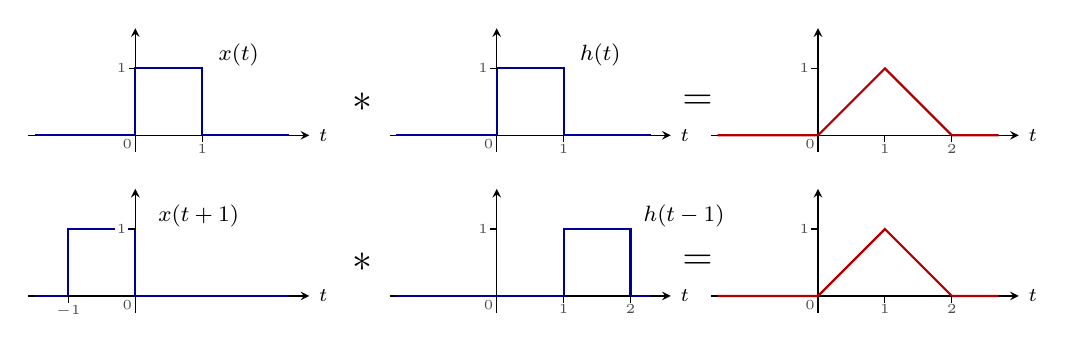
\begin{tikzpicture}[x=0.85cm,y=0.85cm]
  \begin{scope}
    \taxes{-1.6}{2.6}{1.6}{-0.25}
    \draw[sig] (-1.5,0) -- (0,0) -- (0,1) -- (1,1) -- (1,0) -- (2.3,0);
    \xt{1}{1}\yt{1}{1}
    \node[font=\footnotesize,anchor=west] at (1.1,1.2) {$x(t)$};
  \end{scope}
  \opsym{3.4}{0.5}{$\ast$}
  \begin{scope}[shift={(5.4,0)}]
    \taxes{-1.6}{2.6}{1.6}{-0.25}
    \draw[sig] (-1.5,0) -- (0,0) -- (0,1) -- (1,1) -- (1,0) -- (2.3,0);
    \xt{1}{1}\yt{1}{1}
    \node[font=\footnotesize,anchor=west] at (1.1,1.2) {$h(t)$};
  \end{scope}
  \opsym{8.4}{0.5}{$=$}
  \begin{scope}[shift={(10.2,0)}]
    \taxes{-1.6}{3.0}{1.6}{-0.25}
    \draw[res] (-1.5,0) -- (0,0) -- (1,1) -- (2,0) -- (2.7,0);
    \xt{1}{1}\xt{2}{2}\yt{1}{1}
  \end{scope}
  \begin{scope}[shift={(0,-2.4)}]
    \taxes{-1.6}{2.6}{1.6}{-0.25}
    \draw[sig] (-1.5,0) -- (-1,0) -- (-1,1) -- (0,1) -- (0,0) -- (2.3,0);
    \xt{-1}{-1}\yt{1}{1}
    \node[font=\footnotesize,anchor=west] at (0.2,1.2) {$x(t+1)$};
  \end{scope}
  \opsym{3.4}{-1.9}{$\ast$}
  \begin{scope}[shift={(5.4,-2.4)}]
    \taxes{-1.6}{2.6}{1.6}{-0.25}
    \draw[sig] (-1.5,0) -- (1,0) -- (1,1) -- (2,1) -- (2,0) -- (2.3,0);
    \xt{1}{1}\xt{2}{2}\yt{1}{1}
    \node[font=\footnotesize,anchor=west] at (2.05,1.2) {$h(t-1)$};
  \end{scope}
  \opsym{8.4}{-1.9}{$=$}
  \begin{scope}[shift={(10.2,-2.4)}]
    \taxes{-1.6}{3.0}{1.6}{-0.25}
    \draw[res] (-1.5,0) -- (0,0) -- (1,1) -- (2,0) -- (2.7,0);
    \xt{1}{1}\xt{2}{2}\yt{1}{1}
  \end{scope}
\end{tikzpicture}
\caption{上：$[0,1]$ 上的两个方波卷积得 $[0,2]$ 上的三角波。下：$x$ 左移 $1$、$h$ 右移 $1$，起点 $-1+1=0$、终点 $0+2=2$ 都没变，结果仍是同一个三角波。}
\end{figure}

\example{拆成阶跃逐项卷积}{验算 \ref{sub:rect} 小节的例子}{}
\textbf{题目}：用分配律展开 $\big[u(t-1)-u(t-3)\big]\ast\big[u(t+1)-u(t-1)\big]$，验证结果是 $[0,4]$ 上峰值为 $2$ 的三角波。

\point{两个阶跃的卷积。}由 \ref{sub:step} 小节，$u(t)\ast u(t)=\int_{-\infty}^{t}u(\tau)\,\mathrm{d}\tau=t\,u(t)$（斜坡）。再由平移性质（本小节），
\[
u(t-a)\ast u(t-b)=(t-a-b)\,u(t-a-b).
\]
\point{逐项代入。}
\begin{align*}
&u(t-1)\ast u(t+1)-u(t-1)\ast u(t-1)-u(t-3)\ast u(t+1)+u(t-3)\ast u(t-1)\\
&=t\,u(t)-(t-2)\,u(t-2)-(t-2)\,u(t-2)+(t-4)\,u(t-4)\\
&=t\,u(t)-2(t-2)\,u(t-2)+(t-4)\,u(t-4).
\end{align*}
\point{分段核对。}$0<t<2$：$t$；$2<t<4$：$t-2(t-2)=4-t$；$t>4$：$4-t+(t-4)=0$。正是 $[0,4]$ 上、在 $t=2$ 处达到 $2$ 的三角波。这种做法比图解法繁琐得多。

\subsection{一组冲激辨析题}
\example{相乘、积分、卷积}{结果分别是冲激、数、函数}{}
\textbf{题目}：分别求
\[
\text{(1)}\ x(t+2)\,\delta(t-3);\qquad
\text{(2)}\ \int_{-\infty}^{+\infty}x(t+2)\,\delta(t-3)\,\mathrm{d}t;\qquad
\text{(3)}\ x(t+2)\ast\delta(t-3).
\]
\point{(1) 相乘。}用 $x(t)\,\delta(t-t_0)=x(t_0)\,\delta(t-t_0)$，$t_0=3$ 代入 $x(t+2)$ 得 $x(5)$：
\[
x(t+2)\,\delta(t-3)=x(5)\,\delta(t-3).
\]
\point{(2) 积分。}由 (1)，
\[
\int_{-\infty}^{+\infty}x(t+2)\,\delta(t-3)\,\mathrm{d}t=x(5)\int_{-\infty}^{+\infty}\delta(t-3)\,\mathrm{d}t=x(5).
\]
\point{(3) 卷积。}用平移性质（\ref{sub:shift} 小节）：一边加 $3$、一边减 $3$ 可以同时抵消。把 $x(t+2)$ 写成 $x\big((t-1)+3\big)$，
\[
x(t+2)\ast\delta(t-3)=x(t-1)\ast\delta(t)=x(t-1).
\]
最后一步用到任何函数与 $\delta(t)$ 卷积都等于它本身。也可以直接用 $f(t)\ast\delta(t-t_0)=f(t-t_0)$：$x\big((t-3)+2\big)=x(t-1)$。

\begin{remember}
\centering
\renewcommand{\arraystretch}{1.35}
\begin{tabular}{lll}
\toprule
运算 & 结果 & 结果是什么\\
\midrule
$x(t+2)\,\delta(t-3)$ & $x(5)\,\delta(t-3)$ & 一个冲激，强度 $x(5)$\\
$\int_{-\infty}^{+\infty}x(t+2)\,\delta(t-3)\,\mathrm{d}t$ & $x(5)$ & 一个数\\
$x(t+2)\ast\delta(t-3)$ & $x(t-1)$ & 一个函数（把 $x(t+2)$ 右移 $3$）\\
\bottomrule
\end{tabular}
\end{remember}

%==================================================================
\section{LTI 系统的稳定性}\label{sec:stab}
稳定系统的定义：任意有界的输入，都产生有界的输出（有界输入有界输出，bounded-input bounded-output, BIBO）。

\needspace{9\baselineskip}
\begin{remember}
\textbf{定理}（教材第 52 页 2.3.2）：LTI 系统稳定的充要条件是冲激响应绝对可积（离散时绝对可和）：
\[
\int_{-\infty}^{+\infty}|h(t)|\,\mathrm{d}t<+\infty,\qquad
\sum_{n=-\infty}^{+\infty}|h[n]|<+\infty .
\]
\end{remember}

\begin{figure}[H]
\centering
\begin{tikzpicture}[x=1.0cm,y=1.4cm]
  \begin{scope}
    \fill[blue!12] (0,0) -- plot[domain=0:4.3,samples=60] (\x,{exp(-\x)}) -- (4.3,0) -- cycle;
    \taxes{-1}{4.8}{1.6}{-0.2}
    \draw[sig] (-0.9,0) -- (0,0);
    \draw[sig,domain=0:4.3,samples=60] plot (\x,{exp(-\x)});
    \foreach \p in {1,2,3,4}{\xt{\p}{\p}}\yt{1}{1}
    \node[font=\footnotesize,anchor=west] at (0.3,1.35) {$h(t)=e^{-t}u(t)$，面积 $=1$：稳定};
  \end{scope}
  \begin{scope}[shift={(7.2,0)}]
    \shade[left color=blue!15,right color=white] (0,0) rectangle (4.3,1);
    \taxes{-1}{4.8}{1.6}{-0.2}
    \draw[sig] (-0.9,0) -- (0,0) -- (0,1) -- (4.3,1);
    \node[font=\scriptsize] at (4.55,1) {$\cdots$};
    \foreach \p in {1,2,3,4}{\xt{\p}{\p}}\yt{1}{1}
    \node[font=\footnotesize,anchor=west] at (0.3,1.35) {$h(t)=u(t)$，面积 $=+\infty$：不稳定};
  \end{scope}
\end{tikzpicture}
\caption{左：$e^{-t}u(t)$ 绝对可积，系统稳定。右：积分器的 $h(t)=u(t)$ 不绝对可积，系统不稳定；例如输入有界的 $u(t)$，输出 $t\,u(t)$ 无界。}
\end{figure}

\subsection{充分性}
\textbf{要证}：若 $\int_{-\infty}^{+\infty}|h(t)|\,\mathrm{d}t<+\infty$，则对任意有界的 $x(t)$，输出 $y(t)=x(t)\ast h(t)$ 也有界。

\point{证明。}$x(t)$ 有界，即存在 $M$，使得对所有 $t$ 都有 $|x(t)|<M$。用交换律写出 $y(t)$，再把绝对值放进积分号（积分的绝对值不超过绝对值的积分）：
\begin{align*}
|y(t)|=\big|x(t)\ast h(t)\big|
&=\left|\int_{-\infty}^{+\infty}h(\tau)\,x(t-\tau)\,\mathrm{d}\tau\right|\\
&\le\int_{-\infty}^{+\infty}|x(t-\tau)|\,|h(\tau)|\,\mathrm{d}\tau\\
&\le M\int_{-\infty}^{+\infty}|h(\tau)|\,\mathrm{d}\tau<+\infty .
\end{align*}
最后一步：$\int|h|$ 有界，乘以 $M$ 仍有界。离散的情况把积分换成求和，推法相同。

\subsection{必要性}
\textbf{要证}：若 LTI 系统稳定，即对任意 $|x(t)|<M$ 都有 $|y(t)|=|x(t)\ast h(t)|<+\infty$，则 $\int_{-\infty}^{+\infty}|h(t)|\,\mathrm{d}t<+\infty$。

\point{思路：构造一个特殊的有界输入。}既然对\textbf{任意}有界输入输出都有界，就挑一个专门的输入，让某一时刻的输出恰好等于 $\int|h|$。取
\[
x(t)=\begin{cases}+1,& h(-t)>0,\\ -1,& h(-t)<0,\\ \ \ 0,& h(-t)=0,\end{cases}
\]
它显然有界（$|x(t)|\le1$）。这样取，是为了让 $x(\tau)\,h(-\tau)=|h(-\tau)|$ 处处成立。

\point{看 $t=0$ 时刻的输出。}
\begin{align*}
y(0)&=\int_{-\infty}^{+\infty}x(\tau)\,h(0-\tau)\,\mathrm{d}\tau
=\int_{-\infty}^{+\infty}x(\tau)\,h(-\tau)\,\mathrm{d}\tau\\
&=\int_{-\infty}^{+\infty}|h(-\tau)|\,\mathrm{d}\tau
=\int_{-\infty}^{+\infty}|h(\tau)|\,\mathrm{d}\tau .
\end{align*}
系统稳定、输入有界，所以 $y(0)$ 有界，即 $\int_{-\infty}^{+\infty}|h(\tau)|\,\mathrm{d}\tau<+\infty$。证毕。$x(t)$ 的正负号整体取反也可以，此时 $y(0)=-\int|h|$，结论不变。离散的情况取 $x[n]$ 为 $h[-n]$ 的符号，同理得 $y[0]=\sum_k|h[k]|$。

\begin{figure}[H]
\centering
\begin{tikzpicture}[x=0.72cm,y=1.1cm]
  \begin{scope}
    \taxes[\tau]{-6.4}{1.6}{1.35}{-1.2}
    \draw[sig,domain=-6.2:0,samples=160] plot (\x,{exp(0.5*\x)*cos(2*\x r)});
    \draw[sig] (0,0) -- (1.3,0);
    \xtu{-1.571}{-\frac{\pi}{2}}\xt{-3.1416}{-\pi}\xtu{-4.712}{-\frac{3\pi}{2}}\yt{1}{1}\yt{-1}{-1}
    \node[font=\footnotesize,anchor=west] at (-6.3,1.25) {(a) $h(-\tau)$};
  \end{scope}
  \begin{scope}[shift={(9.6,0)}]
    \taxes[\tau]{-6.4}{1.6}{1.35}{-1.2}
    \draw[sig] (-6.2,1) -- (-5.498,1) -- (-5.498,-1) -- (-3.927,-1) -- (-3.927,1) -- (-2.356,1) -- (-2.356,-1) -- (-0.785,-1) -- (-0.785,1) -- (0,1) -- (0,0) -- (1.3,0);
    \xt{-1.571}{-\frac{\pi}{2}}\xt{-3.1416}{-\pi}\xt{-4.712}{-\frac{3\pi}{2}}\yt{1}{1}\yt{-1}{-1}
    \node[font=\footnotesize,anchor=west] at (-6.3,1.25) {(b) $x(\tau)$：取 $h(-\tau)$ 的符号};
  \end{scope}
  \begin{scope}[shift={(4.8,-3.0)}]
    \fill[orange!25] (-6.2,0) -- plot[domain=-6.2:0,samples=160] (\x,{abs(exp(0.5*\x)*cos(2*\x r))}) -- (0,0) -- cycle;
    \taxes[\tau]{-6.4}{1.6}{1.35}{-0.3}
    \draw[res,domain=-6.2:0,samples=160] plot (\x,{abs(exp(0.5*\x)*cos(2*\x r))});
    \draw[res] (0,0) -- (1.3,0);
    \xt{-1.571}{-\frac{\pi}{2}}\xt{-3.1416}{-\pi}\xt{-4.712}{-\frac{3\pi}{2}}\yt{1}{1}
    \node[font=\footnotesize,anchor=west] at (-6.3,1.25) {(c) $x(\tau)\,h(-\tau)=|h(-\tau)|$};
  \end{scope}
\end{tikzpicture}
\caption{取 $h(t)=e^{-t/2}\cos(2t)\,u(t)$ 的例子。(a) $h(-\tau)$ 正负交替；(b) 按它的符号取 $x(\tau)=\pm1$，有界；(c) 两者相乘处处非负，阴影面积就是 $y(0)=\int|h|$。}
\end{figure}

\example{\texorpdfstring{$y(t)=t\,x(t)$}{y(t)=t x(t)} 是否稳定}{不稳定；定理不能用}{}
\textbf{题目}：系统 $y(t)=t\,x(t)$。它的冲激响应 $h(t)=t\,\delta(t)=0\cdot\delta(t)=0$，于是 $\int_{-\infty}^{+\infty}|h(t)|\,\mathrm{d}t=0<+\infty$，由定理得「该系统稳定」。这个推理对吗？

\point{错在用错了定理。}$h(t)$ 的计算没有问题，问题在于：这个系统是线性的，但不是时不变的，\textbf{不是 LTI 系统}，不能用这个定理。实际上它不稳定：输入有界的 $x(t)=1$，输出 $y(t)=t$ 无界。

\begin{remember}
「$\int|h|<+\infty$ 等价于稳定」只对 LTI 系统成立。非 LTI 系统的冲激响应不能唯一确定系统，不能用它判断稳定性。
\end{remember}

%==================================================================
\section{LTI 系统的因果性}\label{sec:causal}
因果性(causality)的定义：输出 $y(t)$ 在 $t_0$ 时刻的值 $y(t_0)$，只由 $t_0$ 之前（包含 $t_0$）的 $x(t)$ 决定。也就是说，输出不会跑到输入的前面。

\needspace{7\baselineskip}
\begin{remember}
\textbf{定理}（教材 2.3.3）：LTI 系统因果的充要条件是
\[
h(t)=0\ \ \text{当}\ t<0\ \text{时},\qquad h[n]=0\ \ \text{当}\ n<0\ \text{时}.
\]
\end{remember}

\point{证明。}写出 $t_0$ 时刻的输出：
\[
y(t_0)=\int_{-\infty}^{+\infty}x(\tau)\,h(t_0-\tau)\,\mathrm{d}\tau .
\]
积分范围是整条 $\tau$ 轴，所以一般来说 $y(t_0)$ 与所有时刻的输入都有关。例外只有一种：$h(t_0-\tau)$ 在 $\tau>t_0$ 时等于 $0$。此时积分只需做到 $t_0$：
\[
y(t_0)=\int_{-\infty}^{t_0}x(\tau)\,h(t_0-\tau)\,\mathrm{d}\tau ,
\]
$y(t_0)$ 只依赖 $\tau\le t_0$ 的输入，系统因果。令 $t=t_0-\tau$，「$\tau>t_0$ 时 $h(t_0-\tau)=0$」等价于「$t<0$ 时 $h(t)=0$」。

反过来，若 $h(t)$ 在 $t<0$ 的某一段上不为 $0$，则 $h(t_0-\tau)$ 在 $\tau>t_0$ 的某一段上不为 $0$；只改动 $t_0$ 之后的输入就能改变 $y(t_0)$，系统不是因果的。

离散的情况：$y[n_0]=\sum_k x[k]\,h[n_0-k]$，「$k>n_0$ 时 $h[n_0-k]=0$」等价于「$n<0$ 时 $h[n]=0$」。

\point{图解法的理解。}卷积要把 $h(t)$ 翻转再平移到 $t_0$。若 $h(t)$ 从 $0$ 才开始有值，翻转后 $h(t_0-\tau)$ 只在 $\tau\le t_0$ 有值，算出的 $y(t_0)$ 只与 $x$ 在 $t_0$ 左边的部分有关。若 $h(t)$ 在 $t<0$ 处多出一截，翻转后就会越过 $t_0$ 伸到右边，$y(t_0)$ 多出了 $t_0$ 之后输入的影响，不再是因果的。

\begin{figure}[H]
\centering
\begin{tikzpicture}[x=0.75cm,y=1.25cm]
  \begin{scope}
    \taxes[\tau]{-1.6}{6.4}{1.45}{-0.2}
    \draw[sig,domain=-1.5:6,samples=80] plot (\x,{0.45+0.15*sin(1.3*\x r)});
    \draw[res,domain=-1.5:3,samples=60] plot (\x,{exp(-(3-\x))});
    \draw[res] (3,1) -- (3,0) -- (6,0);
    \draw[dashed,gray] (3,0) -- (3,1.3);
    \xt{3}{t_0}\yt{1}{1}
    \node[font=\footnotesize,blue!60!black,anchor=west] at (4.2,0.72) {$x(\tau)$};
    \node[font=\footnotesize,red!70!black,anchor=east] at (2.8,1.05) {$h(t_0-\tau)$};
    \node[font=\footnotesize,anchor=west] at (-1.5,1.75) {因果：$h(t)=e^{-t}u(t)$};
  \end{scope}
  \begin{scope}[shift={(10.2,0)}]
    \fill[red!15] (3,0) -- plot[domain=3:6,samples=60] (\x,{exp(-(\x-3))}) -- (6,0) -- cycle;
    \taxes[\tau]{-1.6}{6.4}{1.45}{-0.2}
    \draw[sig,domain=-1.5:6,samples=80] plot (\x,{0.45+0.15*sin(1.3*\x r)});
    \draw[res,domain=-1.5:6,samples=100] plot (\x,{exp(-abs(3-\x))});
    \draw[dashed,gray] (3,0) -- (3,1.3);
    \xt{3}{t_0}\yt{1}{1}
    \node[font=\footnotesize,red!70!black,anchor=north] at (4.7,-0.05) {$\tau>t_0$ 的部分};
    \node[font=\footnotesize,anchor=west] at (-1.5,1.75) {非因果：$h(t)=e^{-|t|}$};
  \end{scope}
\end{tikzpicture}
\caption{左：因果的 $h(t)$ 翻转后只落在 $\tau\le t_0$，$y(t_0)$ 只用到 $t_0$ 之前的输入。右：$h(t)$ 在 $t<0$ 处有值，翻转后伸到 $\tau>t_0$（红色阴影），$y(t_0)$ 用到了 $t_0$ 之后的输入。}
\end{figure}

\point{孤立点不影响结论（连续时间）。}若 $h(t)$ 在 $t>0$ 时有值、在 $t<0$ 处只有个别孤立点不为 $0$（例如 $t=-1$ 处有一个值），定理仍然成立：孤立点不影响积分，按第 06 篇勒贝格的函数相等定义，它和去掉孤立点后的 $h(t)$ 是同一个函数，系统仍是因果的。离散时间没有这个说法：只要某个 $n<0$ 处 $h[n]\ne0$，$y[n_0]$ 就会用到 $n_0$ 之后的输入，系统不是因果的。

\begin{figure}[H]
\centering
\begin{tikzpicture}[x=0.9cm,y=1.25cm]
  \taxes{-2}{4.4}{1.35}{-0.2}
  \draw[sig] (-1.9,0) -- (0,0);
  \draw[sig,domain=0:4.1,samples=60] plot (\x,{exp(-\x)});
  \fill[white] (-1,0) circle (2pt); \draw[sig] (-1,0) circle (2pt);
  \fill[blue!60!black] (-1,0.6) circle (2pt);
  \xt{-1}{-1}\xt{1}{1}\xt{2}{2}\xt{3}{3}\yt{1}{1}
  \node[font=\footnotesize,anchor=west] at (0.4,1.15) {$h(t)$：$t=-1$ 处有一个孤立值};
\end{tikzpicture}
\caption{$t=-1$ 处的孤立值不影响任何积分，这个 $h(t)$ 与 $e^{-t}u(t)$ 是同一个函数，系统仍是因果的。}
\end{figure}

\end{document}
